\section{Radiation from Continuous Sources II}

\subsection{Review of Continuous Distribution Maxwell Solutions}

\begin{center}
    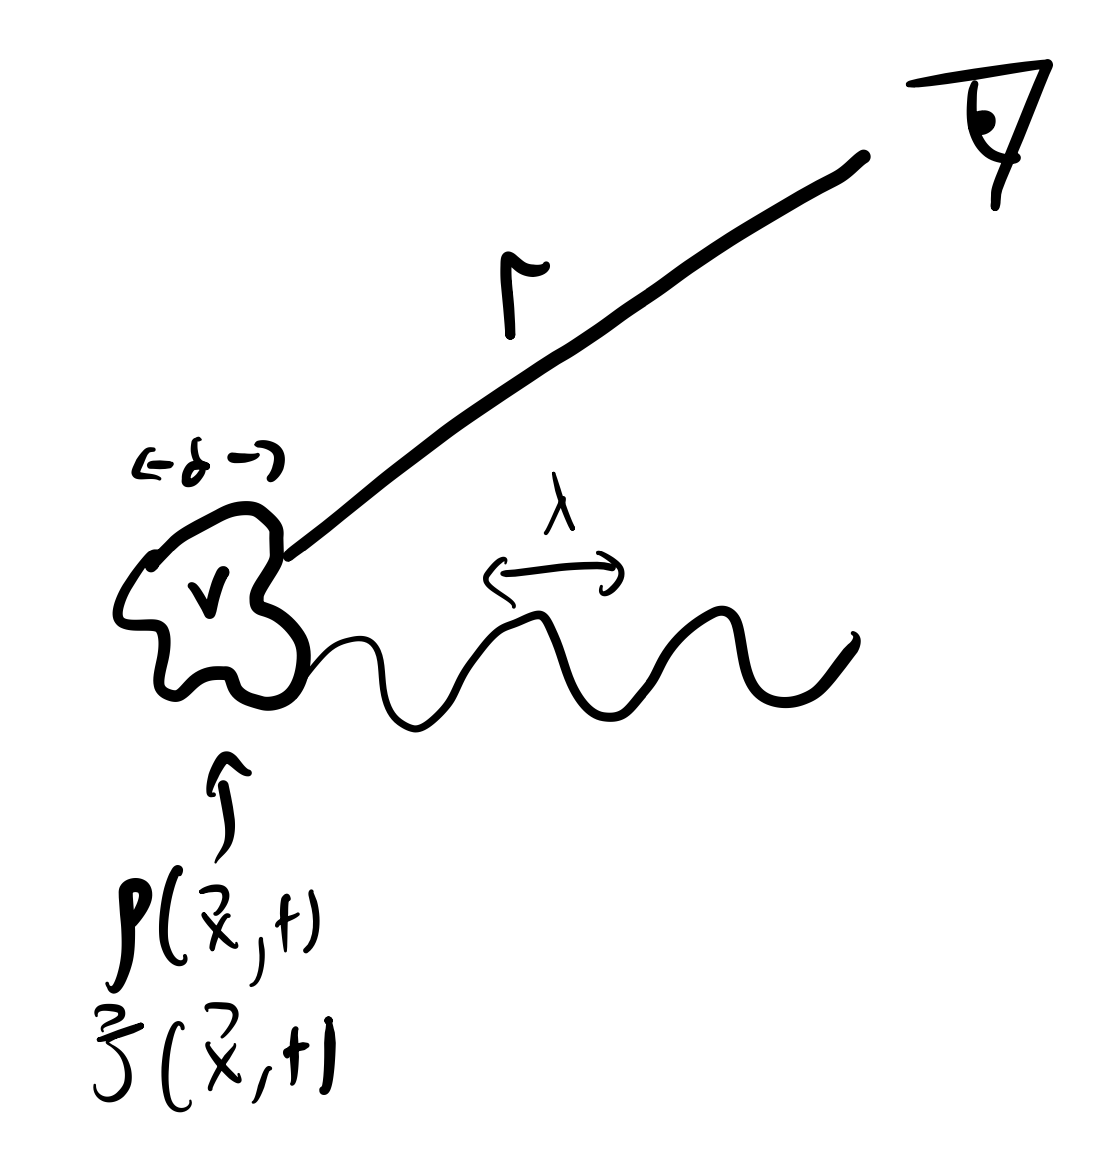
\includegraphics[scale=0.35]{Lectures/Images/lec11-continoussourceradiation.png}
\end{center}

Since Maxwell's equations are linear, we can fourier transform in time and take:
\begin{equation}
    \rho(\v{x}, t) = \rho(\v{x})e^{i\omega t}
\end{equation}\begin{equation}
    \v{J}(\v{x}, t) = \v{J}(\v{x})e^{i\omega t}
\end{equation}
And with the continuity equation:
\begin{equation}
    \dot{\rho} + \nabla \cdot \v{J} = 0
\end{equation}
the two are related by:
\begin{equation}
    i\omega \rho(\v{x}) = \nabla \cdot \v{J}(\v{x})
\end{equation}

Npw, solving Maxwell's equation with these sources, we have:
\begin{equation}
    \v{A}(\v{x}) = \frac{\mu_0}{4\pi}\int d^3\v{x}'\v{J}(\v{x}')\frac{e^{ik\abs{\v{x} - \v{x}'}}}{\abs{\v{x} - \v{x}'}}
\end{equation}
with $k = \frac{\omega}{c} = \frac{2\pi}{\lambda}$. $A_0$ is fixed by the Lorentz gauge condition. From these we get the EM fields:
\begin{equation}
    \v{H} = \frac{1}{\mu_0}\v{B} = \frac{1}{\mu_0}\nabla \times \v{A}
\end{equation}
\begin{equation}
    \v{E} = \frac{iZ_0}{k}\nabla \times \v{H}
\end{equation}
with $Z_0 = \sqrt{\frac{\e_0}{\mu_0}}$.

We studied the long wavelength limit $\lambda \gg d$, and discussed the different regimes where we could place our detector; the near field is where $\abs{\v{x}} \sim d$, the intermediate field is where $\abs{\v{x}} \sim \lambda$, and the far field where $\abs{\v{x}} \gg \lambda$. In this far-field regime:
\begin{equation}
    \v{A}(\v{x}) = \frac{\mu_0}{4\pi}\frac{e^{ikr}}{r}\int_V d^3\v{x}'\v{J}(\v{x}')e^{-ik\hat{\v{n}}\cdot\v{x}'}
\end{equation}
with $r = \abs{\v{x}}$. There is no $r$ dependence left in the integral, but there is an angular dependence through $\hat{\v{n}}\cdot\v{x}'$. In particular this integral depends on $d, \lambda, \theta, \phi$.

\subsection{The Electric Dipole Approximation}
How do we analyze this integral? We can do a power series in the exponential, and get a power series in $\frac{d}{\lambda}$. Doing this:
\begin{equation}
    \int d^3\v{x}' \v{J}(\v{x}')e^{-ik\hat{\v{n}}\cdot\v{x}'} = \sum_{j=0}^\infty \frac{(-ik)^j}{j!}\int d^3\v{x}' \v{J}(\v{x}')(\hat{\v{n}} \cdot \v{x}')^j
\end{equation}
Looking at $j = 0$ - this is the electric dipole approximation:
\begin{equation}
    \v{A}(\v{x}) = \frac{\mu_0}{4\pi}\frac{e^{ikr}}{r}\int d^3\v{x}'\v{J}(\v{x}')
\end{equation}
Why is it called this? Indeed, if we consider:
\begin{equation}
    \gv{\theta} = \int d^3\v{x}' \v{x}(\nabla \cdot \v{J}(\v{x}')) = -\int d^3\v{x}' \v{J}(\v{x}')
\end{equation}
Where in the last equality we have used integration by parts. We also have assumed that the boundary terms vanish - we are in fact interested in the setting where if we exit the region of the source, the currents go to zero. On the other hand, we can replace $\nabla \cdot \v{J}(\v{x}') = i\omega \rho(\v{x}')$ by the continuity equation. With this in mind, let us rewrite the vector potential as:
\begin{equation}
    \v{A}(\v{x}) = -\frac{i\mu_0\omega}{4\pi}\v{p}\frac{e^{ikr}}{r}
\end{equation}
with:
\begin{equation}
    \v{p} = \int d^3\v{x}' \v{x}'\rho(\v{x}')
\end{equation}
So we now understand why this is called the dipole approximation - a time dependent dipole gives rise to this vector potential. From this, we get the magnetic field (as you will check on the problem set):
\begin{equation}
    \v{H} = \frac{ck^2}{4\pi}\hat{\v{n}} \times \v{p}\frac{e{^ikr}}{r}
\end{equation}
and the electric field:
\begin{equation}
    \v{E} = Z_0\v{H} \times \hat{\v{n}}
\end{equation}
There is a nice picture here, namely that the electric field, magnetic field, and $\hat{\v{n}}$ are all perpendicular. EM waves are transverse. From this, we can find the power per solid angle:
\begin{equation}
    \dod{P}{\Omega} = \frac{c^2Z_0}{32\pi^2}k^4\abs{(\hat{\v{n}} \times \v{p}) \times \hat{\v{n}}}^2
\end{equation}
which is why the sky is blue, as the power goes as $\sim \frac{1}{\lambda^4}$ (Rio note: the sky is not purple because of the blackbody spectrum of the sun and the sensitivity of the eyes). Taking the angle between $\v{p}$ and $\hat{\v{n}}$ to be $\sin(\theta)$, we can write the above as:
\begin{equation}
    \dod{P}{\Omega} = \frac{c^2Z_0}{32\pi^2}k^4\abs{\v{p}}^2\sin^2\theta
\end{equation}
Integrating over all angles:
\begin{equation}
    P = \frac{c^2Z_0k^4}{12\pi}\abs{\v{p}}^2
\end{equation}

\subsection{Center-Fed Antenna}
As an example, we can consider an antenna\footnote{As you can tell, I am obsessed with antennas... I will have to stop myself from putting it on the final.}, in particular a center fed antenna:

\begin{center}
    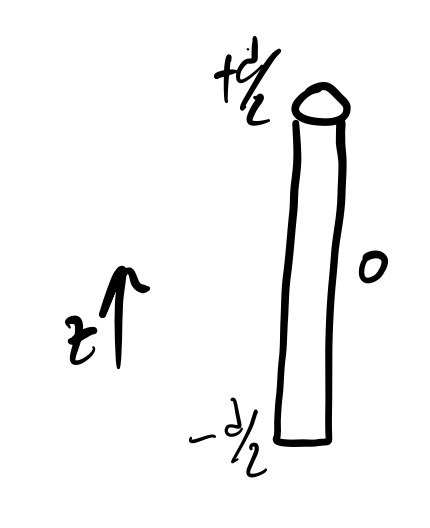
\includegraphics[scale=0.35]{Lectures/Images/lec11-antenna.png}
\end{center}

We can then consider the current density to be:
\begin{equation}
    \v{J}(\v{x}, t) = \hat{\v{z}}J(\v{x}, t) = \hat{z}\delta(x)\delta(y)I(z)e^{-i\omega t}
\end{equation}
With the current:
\begin{equation}
    I(z, t) = \int dxdy J(x, y, z, t)
\end{equation}
We now have the engineering choice for how to craft the current profile; so long as we choose the current to vanish at the edges, anything is ok. For example:

\begin{center}
    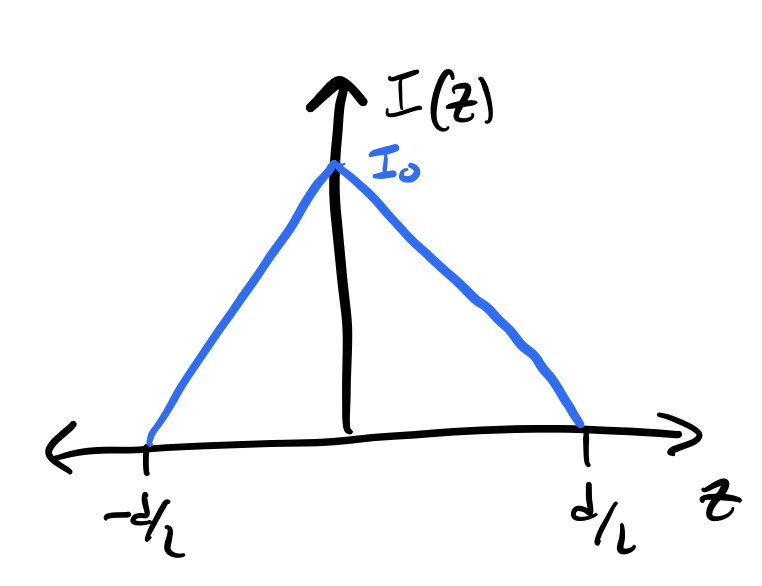
\includegraphics[scale=0.35]{Lectures/Images/lec11-antennacurrent.png}
\end{center}

where the above graphic describes:
\begin{equation}
    I(z) = I_0(1 - \frac{2\abs{z}}{d})
\end{equation}

we can now calculate the radiation from this antenna. We first calculate the $\rho'$:
\begin{equation}
    \rho'(z, t) = \int dxdy \rho(x, y, z, t)
\end{equation}
from the continuity equation:
\begin{equation}
    \dpd{}{t}\rho'(z, t) + \dpd{}{z}I(z, t) = 0 
\end{equation}
after we strip off the time dependence:
\begin{equation}
    \rho'(z) = \begin{cases}
        \frac{2iI_0}{\omega d} & 0 \leq z \leq d/2
        \\ -\frac{2iI_0}{\omega d} & -d/2 \leq z < 0
    \end{cases}
\end{equation}
There is a discontinuity at $z = 0$ as we feed current through the middle here in a non-differentiable way. In a real device the current we supply will be smooth. There is only a $z$-component to the dipole moment:
\begin{equation}
    p_z = \int_{-d/2}^{d/2}dz' z' \rho'(z') = \frac{iI_0d}{2\omega}
\end{equation}
\begin{equation}
    p_x = p_y = 0
\end{equation}
So then we have:
\begin{equation}
    \dod{P}{\Omega} = \frac{Z_0I_0^2}{128\pi^2}(kd)^2\sin^2\theta
\end{equation}
and:
\begin{equation}
    P = \frac{Z_0 I_0^2(kd)^2}{48\pi}
\end{equation}
which is the antenna analogue of the (non-relativistic) Larmor formula (non-relativistic as from our long-wavelength approximation, $\omega$ is small).

\emph{``I'm very happy that people are thinking... unusual experience for me, I guess''} - David Kutasov

\subsection{$j=1$: Antisymmetric/Magnetic Dipole Term}
Now we'll go to $j=1$\footnote{Going to be a long course... we'll be here in August going to $j = 3$. But more seriously, in some fields of physics people do go to very high orders of perturbation theory.}. From our power series formula:
\begin{equation}
    \v{A}(\v{x}) = \frac{\mu_0}{4\pi}\frac{e^{ikr}}{r}(-ik)\int d^3\v{x}'\v{J}(\v{x}')\hat{\v{n}}\cdot\v{\v{x}}'
\end{equation}
So $A_i$ involves $J_i \hat{n}_jx_j'$. It will be useful for us to split $J_ix_j'$ into a symmetric and antisymmetric part:
\begin{equation}
    J_ix_j' = \frac{1}{2}\underbrace{(J_ix_j' + J_jx_i')}_{(ij)} + \frac{1}{2}\underbrace{(J_ix_j' - J_jx_i')}_{[ij]}
\end{equation}
These two terms will have slightly different interpretations in terms of moments of the charge distribution. Let's look at the antisymmetric part first:
\begin{equation}
    J_ix_j' - J_jx_i' = \e_{ijk}(\v{J}\times \v{x}')_k
\end{equation}
Then:
\begin{equation}
    J_i \hat{n}_jx_j' \stackrel{\text{antisym}}{=} \left(\frac{1}{2}\hat{\v{n}} \times (\v{x}' \times \v{J})\right)_i
\end{equation}
Why is this interesting? The magnetic moment density enters the above expression:
\begin{equation}
    \v{M}(\v{x}) = \frac{1}{2}\v{x}\times\v{J}
\end{equation}
where the net magnetic moment is:
\begin{equation}
    \v{m} = \int d^3\v{x}\v{M}(\v{x})
\end{equation}
the bottom line is that the vector potential looks quite simple:
\begin{equation}
    \v{A}(\v{x}) = \frac{ik\mu_0}{4\pi}\hat{\v{n}}\times\v{m}\frac{e^{ikr}}{r}
\end{equation}
with associated magnetic/electric fields:
\begin{equation}
    \v{H} = \frac{1}{4\pi}k^2(\hat{\v{n}} \times \v{m})\times \hat{\v{n}}\frac{e^{ikr}}{r}
\end{equation}
\begin{equation}
    \v{E} = - \frac{Z_0}{4\pi}k^2\hat{\v{n}}\times \v{m}\frac{e^{ikr}}{r}
\end{equation}
so we see the same pattern where both the electric and magnetic fields are orthogonal to the direction of propagation of the wave.

One question we could ask is how is this related to the electric dipole story from earlier? You can read in Kutasov's notes how the two calculations are related by electromagnetic duality.

\subsection{$j=1$: Symmetric/Electric Quadrupole Term}
For the symmetric term, we are interested in the integral:
\begin{equation}
    \frac{1}{2}\int d^3\v{x}'\left[(\hat{\v{n}}\cdot\v{x}')\v{J}(\v{x}')+ (\hat{\v{n}}\cdot\v{J}(\v{x}'))\v{x}'\right]
\end{equation}
By the continuity equation, the above becomes:
\begin{equation}
    -\frac{i\omega}{2}\int d^3\v{x}'\v{x}'(\hat{\v{n}}\cdot\v{x}')\rho(\v{x}')
\end{equation}
From which we obtain:
\begin{equation}
    \v{A}(\v{x}) = -\frac{\mu_0ck^2}{8\pi}\frac{e^{ikr}}{r}\int d^3\v{x}'\v{x}'(\hat{\v{n}}\cdot\v{x}')\rho(\v{x}')
\end{equation}
qualitatively, it does indeed look like one higher moment of the charge distribution, with $\rho(\v{x}')$ giving the total charge/monopole term, $\v{x}'\rho(\v{x}')$ giving the dipole term, and $\v{x}'(\hat{\v{n}}\cdot\v{x}')\rho(\v{x}')$ giving the quadrupole term. The resulting magnetic/electric fields are given by:
\begin{equation}
    \v{H} = \frac{ik}{\mu_0}\hat{\v{n}} \times \v{A}
\end{equation}
\begin{equation}
    \v{E} = \frac{ik}{\mu_0}Z_0(\hat{\v{n}}\times\v{A})\times\hat{\v{n}}
\end{equation}
It is the now-familiar pattern of $\hat{\v{n}}, \v{H}, \v{E}$ being mutually orthogonal in the far-field limit. This will be the starting point of our discussion next time, where we will elaborate on the discussion of quadrapole moments. We could ask why do we care about these - in some situations it could be that not only the total charge/monopole term is zero, but also that the dipole moment also vanishes. In this case the quadrapole could be the leading contribution to the fields and thus to the radiation. In the problem set, you will see an example where this is indeed the case.